% =====================================================================
% SPEAR-Net manuscript  --  target: Earth Science Informatics (Springer)
% ---------------------------------------------------------------------
% This file compiles standalone with pdflatex + bibtex using the generic
% `article` class, so you can build it immediately. To submit to Springer,
% paste the body into the Springer Nature LaTeX template (sn-jnl.cls,
% "pdflatex" / default option) -- the section structure below already
% matches Springer's expected layout (Abstract, Keywords, Introduction,
% ... , Declarations). Replace the \title/\author block with the
% template's \title{}, \author[...]{}, \affil[...]{} macros.
%
% Build:  pdflatex spearnet ; bibtex spearnet ; pdflatex spearnet ; pdflatex spearnet
% =====================================================================
\documentclass[11pt]{article}

\usepackage[utf8]{inputenc}
\usepackage[T1]{fontenc}
\usepackage{lmodern}
\usepackage[hmargin=2.4cm,vmargin=2.6cm]{geometry}
\usepackage{amsmath,amssymb}
\usepackage{graphicx}
\graphicspath{{paper_figures/}{figures/}}
\usepackage{booktabs}
\usepackage{multirow}
\usepackage{array}
\usepackage{siunitx}
\usepackage{xcolor}
\usepackage{caption}
\usepackage{subcaption}
\usepackage[hidelinks]{hyperref}
\usepackage{orcidlink}
\usepackage[numbers,sort&compress]{natbib}
\usepackage{textcomp}

\sisetup{detect-weight=true,detect-family=true}
\newcommand{\best}[1]{\textbf{#1}}
\captionsetup{font=small,labelfont=bf}

\title{\textbf{SPEAR-Net: A Lightweight Spectral-Prior, Recall-Optimized Network for
Global Segmentation of Artisanal and Industrial Mining in Sentinel-2 Imagery}}

\author{%
Author One\,\orcidlink{0000-0000-0000-0000}$^{1,*}$,\quad
Author Two$^{1}$,\quad
Author Three$^{2}$\\[2pt]
\small $^{1}$ Department, University, City, Country\\
\small $^{2}$ Department, University, City, Country\\
\small $^{*}$ Corresponding author: \texttt{corresponding@email.edu}
}
\date{}

\begin{document}
\maketitle

% =====================================================================
\begin{abstract}
\noindent
Artisanal and small-scale mining (ASM), which is frequently unregulated or illegal, is
spatially fragmented and spectrally similar to bare soil, rock and turbid water, so it is
routinely missed by segmentation models and confused with natural background; at the same
time, continental-to-global monitoring on constrained or free-tier hardware calls for
compact, low-latency networks. We present \emph{SPEAR-Net}, a lightweight
(\num{1.06}\,M-parameter, \textless\,\num{0.65}\,GFLOPs at $256^2$) semantic-segmentation
network for mapping mining on Sentinel-2 imagery. SPEAR-Net computes four
physically-informed spectral indices---NDVI, MNDWI, NDTI and BSI---on the fly from the
six visible-to-shortwave-infrared bands and fuses them as an explainable spatial prior
that steers the encoder-decoder toward physically plausible mining surfaces, and it is
trained with a recall-weighted, boundary-aware objective designed for small, fragmented
targets. We train and evaluate on a globally distributed, expert-verified dataset that
provides an explicit \emph{artisanal-versus-industrial} label. On the three-class task
(background / artisanal / industrial), SPEAR-Net attains \num{0.64} mean IoU at
\num{0.78} recall---comparable to U-Net, DeepLabV3+ and U-Net++ (\num{0.653}--\num{0.655}
mIoU) while using \num{20}--\num{25}$\times$ fewer parameters and \num{30}--\num{60}$\times$
fewer floating-point operations. Component analysis shows that the full spectral prior
improves the industrial class over an RGB-only variant, and that the recall-oriented
objective raises recall from \num{0.71} to \num{0.78} while recovering both mining scales
without collapsing to background. In a leave-one-region-out experiment (holding out Asia
and Oceania), the model does not degrade on unseen continents. SPEAR-Net offers a
favourable accuracy--efficiency operating point for large-area, resource-constrained
mining surveillance.
\end{abstract}

\vspace{4pt}
\noindent\textbf{Keywords:} artisanal and small-scale mining; semantic segmentation;
Sentinel-2; spectral indices; lightweight deep learning; recall-optimized loss;
geographic generalization.

% =====================================================================
\section{Introduction}\label{sec:intro}

Mining reshapes land surfaces at a global scale, and its most policy-sensitive form
---artisanal and small-scale mining (ASM)---is often informal or illegal, environmentally
damaging, and difficult to govern precisely because it is small, transient and spatially
scattered \citep{maus2022global,gallwey2020asm}. Earth-observation satellites such as
Sentinel-2 \citep{drusch2012sentinel2} provide the frequent, free, multispectral coverage
needed to monitor mining over large areas, and semantic segmentation of satellite imagery
is the natural tool for delineating mining footprints. Yet a recurring failure mode is
reported across sensors and architectures: small, fragmented, low-density mining is
under-detected and confused with bare soil, rock and water, producing low recall and false
alarms \citep{gallwey2020asm,balaniuk2020mining}. This failure disproportionately affects
ASM, which is the very class of greatest regulatory interest.

Two practical constraints compound the scientific difficulty. First, the strongest public
mining annotations are heavy: pixel-wise datasets can reach tens of gigabytes and hundreds
of thousands of tiles, which is impractical on the free-tier accelerators (e.g. single
consumer or cloud GPUs with modest memory) available to many operational and academic
users. Second, prior work rarely reports the computational cost of the proposed model,
even though deployability---parameter count, floating-point operations (FLOPs) and
latency---is decisive for continental-scale or edge inference.

We argue that these constraints can be turned into design principles. We build on a
globally distributed, expert-verified mining dataset whose annotation package is compact
(tens of megabytes) and whose imagery is fetched on demand from an open archive, so a
representative subset trains comfortably on free-tier hardware. Crucially, this dataset
carries an explicit, manually validated \emph{scale} attribute (artisanal vs.\ industrial),
making the small-scale/illegal-prone class \emph{trainable} rather than a near-empty pixel
category. Fetching the raw bands ourselves restores the near-infrared (NIR) and
shortwave-infrared (SWIR) channels, enabling a physically grounded spectral prior, and the
global footprint enables a geographic generalization protocol seldom evaluated in the
mining literature.

Concretely, we make the following contributions.
\begin{enumerate}
\item \textbf{A compact model at near-parity accuracy.} We propose SPEAR-Net, a
\num{1.06}\,M-parameter, sub-GFLOP segmentation network that \emph{matches} strong
convolutional baselines (U-Net, DeepLabV3+, U-Net++) to within \textasciitilde\,\num{1.3}
mIoU points, at comparable recall, using \num{20}--\num{25}$\times$ fewer parameters and
\num{30}--\num{60}$\times$ fewer FLOPs (Section~\ref{sec:results-main}).
\item \textbf{A physically-informed spectral prior (PISP).} Four remote-sensing indices are
computed on the fly and fused as an explainable spatial prior. Replacing the full six-band
prior with an RGB-only variant reduces performance, quantifying the value of the NIR/SWIR
bands (Section~\ref{sec:results-ablation}).
\item \textbf{A recall-oriented objective for fragmented targets.} A compound
Dice--Tversky--focal loss with a boundary/edge stream raises recall from \num{0.71} to
\num{0.78} and recovers both mining scales without background collapse.
\item \textbf{Artisanal-versus-industrial mapping on verified global labels}, together with
a \emph{leave-one-region-out} generalization protocol that is rarely reported for mining
segmentation (Section~\ref{sec:results-gen}).
\end{enumerate}

We report single-run results and deliberately frame our claims as \emph{parity plus
efficiency} rather than accuracy superiority; where component differences are within the
margin one would expect from run-to-run variation, we say so explicitly. All code, configs
and the data-preparation pipeline are released for reproducibility.

% =====================================================================
\section{Related work}\label{sec:related}

\paragraph{Mining and ASM mapping from satellite imagery.}
Global inventories of mining land use have been assembled from manual and semi-automatic
interpretation of optical imagery \citep{maus2022global} and, more recently, from
high-resolution satellite mapping \citep{tang2023mining}. Deep learning is increasingly
applied to mining footprints: \citet{saputra2025multimodal} performed multi-modal semantic
segmentation of mining land covers across 37 sites worldwide, and
\citet{balaniuk2020mining} addressed mining and tailings-dam detection at national scale.
Multi-class monitoring systems such as MineCam combine segmentation and change detection
over annotated mine components \citep{jablonska2024minecam}. For ASM specifically,
\citet{gallwey2020asm} trained a multispectral convolutional network to detect small-scale
mining in Ghana, \citet{ngom2020senegal} mapped artisanal gold mining in Senegal from
Sentinel-2 data, \citet{couttenier2022asm} mapped ASM over 1.75 million~km$^2$ of West
Africa with a segmentation network, and \citet{fonseca2024asm} improved ASM detection with
spectral--textural segmentation of Landsat time series. A recent systematic review of ASM
mapping \citep{nursamsi2024review} concludes that approaches which succeed locally do not
yet scale to regional or global monitoring. A consistent theme across these studies is that
fragmented, low-density mining is hard to recover and easily confused with spectrally
similar background, motivating methods that inject physical priors and explicitly optimize
recall; moreover, none of them reports the computational cost of the deployed model, which
is central here.

\paragraph{Semantic segmentation architectures.}
Since fully convolutional networks established dense prediction \citep{long2015fcn},
encoder--decoder networks with skip connections, epitomized by U-Net
\citep{ronneberger2015unet} and its successors U-Net++ \citep{zhou2019unetpp} and
Attention U-Net \citep{oktay2018attentionunet}, have remained strong baselines, as have
context-aggregation designs such as PSPNet \citep{zhao2017pspnet}, atrous
encoder--decoders such as DeepLabV3+ \citep{chen2018deeplabv3plus} and transformer
segmenters such as SegFormer \citep{xie2021segformer}. These models are accurate but
parameter-heavy (tens of millions of weights). Efficiency-oriented backbones---MobileNetV2/V3
\citep{sandler2018mobilenetv2,howard2019mobilenetv3}, EfficientNet
\citep{tan2019efficientnet} and depthwise-separable convolutions
\citep{chollet2017xception}---enable compact segmenters, but their accuracy--efficiency
trade-off for fine-grained mining segmentation has not been systematically reported.

\paragraph{Spectral indices and prior-guided attention.}
Normalized-difference indices such as NDVI \citep{rouse1974ndvi} and MNDWI
\citep{xu2006mndwi}, and soil/turbidity indices such as BSI \citep{rikimaru2002bsi}, encode
domain knowledge about vegetation, water and bare ground. In mining remote sensing they are
typically used as hand-crafted features for classical classifiers, or fed as raw extra
channels, rather than as a \emph{learned}, spatially explicit attention prior inside a
modern segmentation network. We revisit these indices as a differentiable, explainable gate.

\paragraph{Imbalanced-segmentation losses.}
Region-overlap losses (Dice \citep{milletari2016vnet,sudre2017generaliseddice}, Tversky
\citep{salehi2017tversky}), the focal loss \citep{lin2020focal} and boundary-aware losses
\citep{kervadec2021boundary} were introduced to counter class imbalance and to sharpen
object boundaries. We combine them into a single recall-oriented objective tailored to the
small, fragmented artisanal class.

% =====================================================================
\section{Materials and methods}\label{sec:methods}

\subsection{Dataset}\label{sec:data}
We use a globally distributed, machine-learning-ready mining dataset
\citep{jasansky2024dataset} that reconciles and manually re-validates polygons derived from
\citet{maus2022global} and \citet{tang2023mining}. The annotation package is compact and
provides, per site, the exact Sentinel-2 scene reference, mask polygons, a train/validation/
test split, and two metadata attributes: a mine-type label (surface, placer, underground,
brine/evaporation) and a \emph{scale} label---\emph{artisanal} versus \emph{industrial}---
which is the attribute of primary interest here. The dataset contains
\num{1514} annotated tiles, of which \num{329} are labelled artisanal and \num{1185}
industrial (Table~\ref{tab:data}). Reported annotation quality on the held-out test set is
high (precision \textgreater\,\num{0.99}, recall \textgreater\,\num{0.95}), which makes the
scale attribute reliable enough to serve as a training target. The geographic distribution
of the sites is shown in Fig.~\ref{fig:map}; both scale classes span South America, Africa,
Asia and Oceania, which is what later enables the leave-one-region-out protocol of
Section~\ref{sec:results-gen}.

\begin{figure}[t]
\centering
\includegraphics[width=\linewidth]{fig_dataset_map}
\caption{Geographic distribution of the \num{1514} annotated mining sites, coloured by the
manually verified scale attribute (artisanal vs.\ industrial). The global footprint spans
five continents and underpins the leave-one-region-out generalization protocol.}
\label{fig:map}
\end{figure}

\begin{table}[t]
\centering
\caption{Composition of the mining dataset used in this study. The scale attribute
(artisanal/industrial) is the target for the three-class task.}
\label{tab:data}
\small
\begin{tabular}{lccc}
\toprule
Attribute & Value & Count & Share \\
\midrule
\multirow{2}{*}{Scale} & Artisanal  & \num{329}  & \num{21.7}\,\% \\
                       & Industrial & \num{1185} & \num{78.3}\,\% \\
\midrule
\multirow{4}{*}{Mine type} & Surface & \num{1245} & \num{82.2}\,\% \\
                           & Placer  & \num{187}  & \num{12.4}\,\% \\
                           & Brine/evaporation & \num{58} & \num{3.8}\,\% \\
                           & Underground & \num{24} & \num{1.6}\,\% \\
\midrule
\multirow{3}{*}{Split} & Train & \num{890} & --- \\
                       & Validation & \num{201} & --- \\
                       & Test  & \num{116} & --- \\
\bottomrule
\end{tabular}
\end{table}

\subsection{Imagery retrieval and chipping}\label{sec:prep}
Sentinel-2 Level-2A surface-reflectance imagery is retrieved on demand from an open cloud
archive \citep{planetarycomputer}. For each tile we resolve the corresponding scene by its
grid tile and acquisition date and load six bands---blue (B2), green (B3), red (B4),
near-infrared (B8), and shortwave-infrared SWIR1 (B11) and SWIR2 (B12)---resampled to a
common \SI{10}{\meter} grid over a $2048\times2048$ window centred on the site. Mask
polygons are rasterized onto the same grid and coordinate reference system. Windows are cut
into non-overlapping $256\times256$ chips; mining-containing chips are kept, together with a
sampled fraction of mining-free chips as negatives. To keep the pipeline light, we retrieve
all artisanal tiles and a matched subset of industrial tiles, yielding \num{15271} chips
across the predefined splits. Reflectance digital numbers are scaled by \num{10000} to
approximate surface reflectance $\rho\in[0,1]$. No further preprocessing is applied; the
spectral indices below are computed inside the data loader.

\subsection{Overview of SPEAR-Net}\label{sec:arch}
SPEAR-Net is an encoder--decoder segmenter with three additions targeted at fine-grained
mining: (i) an ImageNet-pretrained lightweight encoder whose stem is adapted from three to
six input bands; (ii) a physically-informed spectral prior (PISP) that modulates the
decoder skip connections; and (iii) a segmentation head paired with an auxiliary
edge/boundary head for deep supervision. Figure~\ref{fig:arch} shows the architecture.

\begin{figure}[t]
\centering
% Vector figure produced by architecture.tex (compile it separately to
% architecture.pdf after dropping the real thumbnails into paper_figures/).
\includegraphics[width=\linewidth]{architecture}
\caption{SPEAR-Net architecture. Four physically-informed spectral indices (NDVI, MNDWI,
NDTI, BSI) are computed on the fly and passed through a small gate to a single spatial
attention map $A$. In the depthwise-separable U-Net decoder each encoder skip is first
\emph{gated} by the attention, $F'=F\odot(1+\alpha A_{\downarrow})$ with a per-scale
learnable $\alpha$, and then \emph{concatenated} (\,\textcircled{\scriptsize C}\,) with the
upsampled decoder feature; the deepest feature (s5) is the ungated bottleneck. A
segmentation head and an auxiliary edge head (deep supervision) produce the outputs, and
the compound loss compares them against the ground-truth mask and its Sobel boundary.}
\label{fig:arch}
\end{figure}

\paragraph{Encoder.}
We use MobileNetV3-Small \citep{howard2019mobilenetv3} pretrained on ImageNet
\citep{deng2009imagenet} as a feature extractor, returning multi-scale features at strides
$2$ to $32$. To accept six bands, the first convolution is expanded from three to six input
channels, initializing the additional NIR/SWIR filters by tiling and rescaling the
pretrained RGB filters so that pretrained low-level features are preserved. The decoder is a
U-Net-style path built from depthwise-separable convolution blocks
\citep{chollet2017xception} with channel widths $\{128,64,48,32\}$, progressively upsampling
and fusing gated skip features.

\subsection{Physically-informed spectral prior (PISP)}\label{sec:pisp}
From the reflectance bands
$\rho_{\mathrm{B}},\rho_{\mathrm{G}},\rho_{\mathrm{R}},\rho_{\mathrm{NIR}},
\rho_{\mathrm{SWIR1}},\rho_{\mathrm{SWIR2}}$ we compute four indices that encode the
dominant visual cues of mining---loss of vegetation, presence of ponds and turbid water,
and exposed bare ground/tailings:
\begin{align}
\mathrm{NDVI}  &= \frac{\rho_{\mathrm{NIR}}-\rho_{\mathrm{R}}}{\rho_{\mathrm{NIR}}+\rho_{\mathrm{R}}}, \label{eq:ndvi}\\[2pt]
\mathrm{MNDWI} &= \frac{\rho_{\mathrm{G}}-\rho_{\mathrm{SWIR1}}}{\rho_{\mathrm{G}}+\rho_{\mathrm{SWIR1}}}, \label{eq:mndwi}\\[2pt]
\mathrm{NDTI}  &= \frac{\rho_{\mathrm{R}}-\rho_{\mathrm{G}}}{\rho_{\mathrm{R}}+\rho_{\mathrm{G}}}, \label{eq:ndti}\\[2pt]
\mathrm{BSI}   &= \frac{(\rho_{\mathrm{SWIR1}}+\rho_{\mathrm{R}})-(\rho_{\mathrm{NIR}}+\rho_{\mathrm{B}})}
                       {(\rho_{\mathrm{SWIR1}}+\rho_{\mathrm{R}})+(\rho_{\mathrm{NIR}}+\rho_{\mathrm{B}})}. \label{eq:bsi}
\end{align}
Stacking the four indices gives a tensor
$\mathbf{P}\in\mathbb{R}^{4\times H\times W}$ (NDVI is vegetation
\citep{rouse1974ndvi}, MNDWI water \citep{xu2006mndwi}, NDTI turbidity, BSI bare soil
\citep{rikimaru2002bsi}). A small convolutional gate maps $\mathbf{P}$ to a single-channel
spatial attention map,
\begin{equation}
\mathbf{A} = \sigma\!\big(\, g(\mathbf{P}) \,\big),\qquad
g(\mathbf{P}) = \mathrm{Conv}_{1\times1}\!\big(\phi\big(\mathrm{DWConv}_{3\times3}(\phi(\mathrm{Conv}_{1\times1}(\mathbf{P})))\big)\big),
\label{eq:gate}
\end{equation}
where $\phi$ is a batch-normalized ReLU, $\mathrm{DWConv}$ a depthwise convolution and
$\sigma$ the logistic function, so $\mathbf{A}\in(0,1)^{1\times H\times W}$. The map is
applied multiplicatively to each decoder skip feature $\mathbf{F}_s$ at scale $s$:
\begin{equation}
\mathbf{F}'_s = \mathbf{F}_s \odot \big(1 + \alpha_s\, \mathbf{A}_{\downarrow s}\big),
\label{eq:apply}
\end{equation}
where $\mathbf{A}_{\downarrow s}$ is $\mathbf{A}$ bilinearly resized to the resolution of
scale $s$, $\alpha_s$ is a learnable per-scale scalar, and $\odot$ is broadcast elementwise
multiplication. The residual form $1+\alpha_s\mathbf{A}$ lets the network fall back to the
ungated feature when the prior is uninformative. Because $\mathbf{A}$ is a single explicit
map derived from named indices, it is directly interpretable as ``where the spectral
evidence for mining is strongest''. As an ablation we also consider a simpler
\emph{concatenation} variant, in which $\mathbf{P}$ is appended to the input bands and
linearly projected back to six channels, and an \emph{RGB-only} variant in which the same
gate is driven by three colour indices computed from the visible bands alone.

\subsection{Recall-weighted, boundary-aware objective}\label{sec:loss}
Let $p_{c}$ and $g_{c}$ denote the predicted probability and one-hot ground truth for class
$c$, and let $\mathcal{C}^{+}$ be the set of classes present in a batch. We combine four
terms. A generalized Dice term \citep{sudre2017generaliseddice},
\begin{equation}
\mathcal{L}_{\mathrm{Dice}} = 1 - \frac{1}{|\mathcal{C}^{+}|}\sum_{c\in\mathcal{C}^{+}}
\frac{2\sum_i p_{c,i} g_{c,i} + \epsilon}{\sum_i p_{c,i} + \sum_i g_{c,i} + \epsilon},
\label{eq:dice}
\end{equation}
averaged \emph{only over present classes} to avoid a spurious penalty that would otherwise
drive the network toward the majority (background) class. A Tversky term
\citep{salehi2017tversky} with $\alpha<\beta$ penalizes false negatives more than false
positives, directly favouring recall of the rare classes:
\begin{equation}
\mathcal{L}_{\mathrm{Tv}} = 1 - \frac{1}{|\mathcal{C}^{+}|}\sum_{c\in\mathcal{C}^{+}}
\frac{\sum_i p_{c,i} g_{c,i}}
     {\sum_i p_{c,i} g_{c,i} + \alpha\sum_i p_{c,i}(1-g_{c,i}) + \beta\sum_i (1-p_{c,i}) g_{c,i}}.
\label{eq:tversky}
\end{equation}
A class-weighted focal term \citep{lin2020focal} supplies a per-pixel gradient that focuses
on hard, rare-class pixels,
\begin{equation}
\mathcal{L}_{\mathrm{F}} = -\frac{1}{N}\sum_{i} w_{y_i}\, (1-p_{y_i,i})^{\gamma}\, \log p_{y_i,i},
\label{eq:focal}
\end{equation}
with $w$ the inverse-frequency class weights and $\gamma$ the focusing parameter. Finally, a
boundary term concentrates a cross-entropy penalty on the ground-truth object boundaries
$\mathbf{B}$ (the Sobel edges of the target mask), and an auxiliary head predicts those
boundaries directly:
\begin{equation}
\mathcal{L}_{\mathrm{B}} = \frac{\sum_i \mathbf{B}_i\, \mathrm{CE}_i}{\sum_i \mathbf{B}_i + \epsilon},
\qquad
\mathcal{L}_{\mathrm{E}} = \mathrm{BCE}\big(\sigma(\hat{\mathbf{e}}),\, \mathbf{B}\big).
\label{eq:boundary}
\end{equation}
The total objective is
\begin{equation}
\mathcal{L} = \lambda_{\mathrm{D}}\mathcal{L}_{\mathrm{Dice}}
            + \lambda_{\mathrm{T}}\mathcal{L}_{\mathrm{Tv}}
            + \lambda_{\mathrm{F}}\mathcal{L}_{\mathrm{F}}
            + \lambda_{\mathrm{B}}\mathcal{L}_{\mathrm{B}}
            + \lambda_{\mathrm{E}}\mathcal{L}_{\mathrm{E}}.
\label{eq:total}
\end{equation}

\subsection{Training details}\label{sec:training}
Unless stated otherwise we use
$\lambda_{\mathrm{D}}=\lambda_{\mathrm{T}}=\lambda_{\mathrm{F}}=1$,
$\lambda_{\mathrm{B}}=\lambda_{\mathrm{E}}=0.5$, Tversky $(\alpha,\beta)=(0.3,0.7)$, and
focal $\gamma=2$. Class weights $w$ are estimated by median-frequency balancing on a random
sample of masks, and chips containing the rare (artisanal) class are oversampled. Models are
trained with AdamW \citep{loshchilov2019adamw} at a base learning rate of
$3\times10^{-4}$, weight decay $10^{-4}$, a cosine schedule \citep{loshchilov2017sgdr} with a
three-epoch linear warm-up, mixed-precision, gradient clipping at norm $1$, batch size
$10$, and $40$ epochs. Implementation uses PyTorch \citep{paszke2019pytorch}; convolutional
baselines use the implementations of \citet{iakubovskii2019smp} with ResNet-34 encoders
\citep{he2016resnet} and the same six-band input, loss and schedule for a controlled
comparison. Training used a single NVIDIA A100
GPU; the model also fits and trains within the memory of a free-tier 16\,GB accelerator.

\subsection{Evaluation}\label{sec:eval}
With $\mathrm{TP}_c$, $\mathrm{FP}_c$ and $\mathrm{FN}_c$ the pixel-level true positives,
false positives and false negatives of class $c$ accumulated over the evaluation set, we
report the per-class Intersection-over-Union and recall,
\begin{equation}
\mathrm{IoU}_c \;=\; \frac{\mathrm{TP}_c}{\mathrm{TP}_c+\mathrm{FP}_c+\mathrm{FN}_c},
\qquad
R_c \;=\; \frac{\mathrm{TP}_c}{\mathrm{TP}_c+\mathrm{FN}_c},
\label{eq:iou}
\end{equation}
and their means over the $C$ classes present in the ground truth,
\begin{equation}
\mathrm{mIoU} \;=\; \frac{1}{C}\sum_{c=1}^{C}\mathrm{IoU}_c,
\qquad
\overline{R} \;=\; \frac{1}{C}\sum_{c=1}^{C} R_c .
\label{eq:miou}
\end{equation}
To probe the field-wide small-object failure directly, we additionally compute an
\emph{area-stratified recall} at the object level. Let
$\mathcal{K}_b=\{K_1,\dots,K_{n_b}\}$ be the connected components of the foreground ground
truth whose pixel area falls in bin $b\in\{$small $<32^2$, medium, large $\geq96^2\}$; a
component counts as recovered if at least one of its pixels is predicted with the correct
class, giving
\begin{equation}
R^{\mathrm{area}}_b \;=\; \frac{1}{n_b}\,
\bigl|\{\,K\in\mathcal{K}_b : \hat{Y}\cap K \neq \varnothing \,\}\bigr| ,
\label{eq:areastrat}
\end{equation}
where $\hat{Y}$ denotes the set of pixels predicted as the component's class. This metric
is deliberately lenient at the pixel level so that it isolates \emph{detection} of a site
from delineation quality. Efficiency is reported as parameter count and
multiply--accumulate operations (GFLOPs) at $256^2$ input. For geographic generalization
we assign each chip to a continent from its centroid and perform a leave-one-region-out
experiment, training with two continents held out and testing on them.

% =====================================================================
\section{Results}\label{sec:results}

\subsection{Comparison with baselines}\label{sec:results-main}
Table~\ref{tab:main} reports the three-class results at full budget (\num{40} epochs, full
data). The convolutional baselines obtain \num{0.653}--\num{0.655} mIoU with
\num{22}--\num{26}\,M parameters and \num{16}--\num{37} GFLOPs. SPEAR-Net obtains
\num{0.642} mIoU (concatenation prior) and \num{0.639} mIoU (gate prior)---within
\textasciitilde\,\num{0.013} mIoU of the best baseline, i.e.\ approximately \num{98}\,\% of
its accuracy---at \num{1.06}\,M parameters and $\leq$\,\num{0.61} GFLOPs, a
\num{20}--\num{25}$\times$ reduction in parameters and a \num{30}--\num{60}$\times$
reduction in FLOPs. Recall is comparable (\num{0.784} vs.\ \num{0.793}), and per-class IoU
is balanced across the artisanal (\num{0.52}) and industrial (\num{0.50}) classes,
indicating that both scales are recovered rather than one dominating. Given the
order-of-magnitude efficiency gain at essentially matched accuracy, SPEAR-Net occupies a
favourable operating point for large-area, resource-constrained inference. This trade-off
is visualized in Fig.~\ref{fig:efficiency}: the lightweight variants form a cluster within
\num{0.02} mIoU of the baselines while sitting more than an order of magnitude to the left
on the (logarithmic) parameter axis.

\begin{figure}[t]
\centering
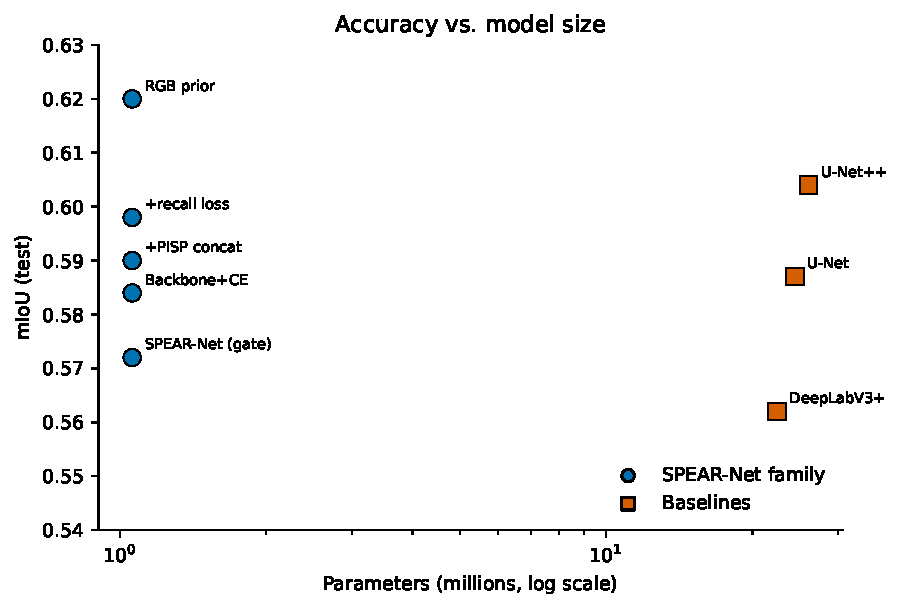
\includegraphics[width=0.72\linewidth]{fig_efficiency}
\caption{Accuracy--efficiency trade-off: mIoU versus parameter count (logarithmic axis).
SPEAR-Net variants (circles) attain approximately \num{98}\,\% of the best baseline's mIoU
at \num{20}--\num{25}$\times$ fewer parameters (squares: U-Net, DeepLabV3+, U-Net++).}
\label{fig:efficiency}
\end{figure}

\begin{table}[t]
\centering
\caption{Three-class segmentation (background / artisanal / industrial) on the test-time
validation set; \num{40} epochs, full data, single run. Best value per column in
\textbf{bold}. Efficiency is measured at $256^2$ input.}
\label{tab:main}
\small
\setlength{\tabcolsep}{5pt}
\begin{tabular}{l ccc cc rr}
\toprule
Method & mIoU & Recall & \multicolumn{3}{c}{Per-class IoU} & Params & GFLOPs\\
\cmidrule(lr){4-6}
 & & & bg & artisanal & industrial & (M) & \\
\midrule
U-Net \citep{ronneberger2015unet}          & \best{0.655} & \best{0.793} & 0.902 & \best{0.553} & 0.511 & 24.45 & 16.06 \\
U-Net++ \citep{zhou2019unetpp}             & 0.655 & 0.762 & \best{0.908} & 0.524 & \best{0.534} & 26.09 & 37.27 \\
DeepLabV3+ \citep{chen2018deeplabv3plus}   & 0.653 & 0.783 & 0.903 & 0.550 & 0.506 & 22.45 & 16.14 \\
\midrule
SPEAR-Net (concat prior)                   & 0.642 & 0.764 & 0.904 & 0.517 & 0.504 & \best{1.06} & \best{0.53} \\
SPEAR-Net (gate prior)                     & 0.639 & 0.784 & 0.901 & 0.515 & 0.500 & 1.06 & 0.61 \\
\bottomrule
\end{tabular}
\end{table}

\subsection{Component analysis (ablation)}\label{sec:results-ablation}
Table~\ref{tab:ablation} isolates each component of SPEAR-Net under the identical training
budget. Adding the recall-weighted objective to the plain backbone raises recall from
\num{0.714} to \num{0.748} and lifts the harder industrial class (IoU
\num{0.459}$\rightarrow$\num{0.487}). Adding the spectral prior further improves the
industrial class. Comparing the two integration modes, concatenation and the learned gate
perform \emph{comparably} on mIoU (\num{0.642} vs.\ \num{0.639}); the gate yields the higher
recall (\num{0.784}), which we prioritize for the detection of easily-missed artisanal
sites, whereas concatenation gives the marginally higher mIoU at slightly lower cost.
Replacing the full six-band spectral prior with an RGB-only prior reduces mIoU by
\num{0.011} and industrial IoU by \num{0.035}, confirming the contribution of the NIR/SWIR
bands (Eqs.~\ref{eq:ndvi}--\ref{eq:bsi}). We emphasize that the spread among the lightweight
variants is small ($\approx$\,\num{0.01} mIoU) and consistent with run-to-run variation; we
therefore treat these components as comparable rather than strictly ordered, and interpret
the gate as a recall-oriented design choice rather than an accuracy improvement. The
per-variant breakdown is summarized graphically in Fig.~\ref{fig:ablbars}; the background
class ($\mathrm{IoU}\approx0.90$ for every variant) is omitted from the chart so that the
axis resolves the differences on the two mining classes, and is reported in
Table~\ref{tab:ablation} instead.

\begin{figure}[t]
\centering
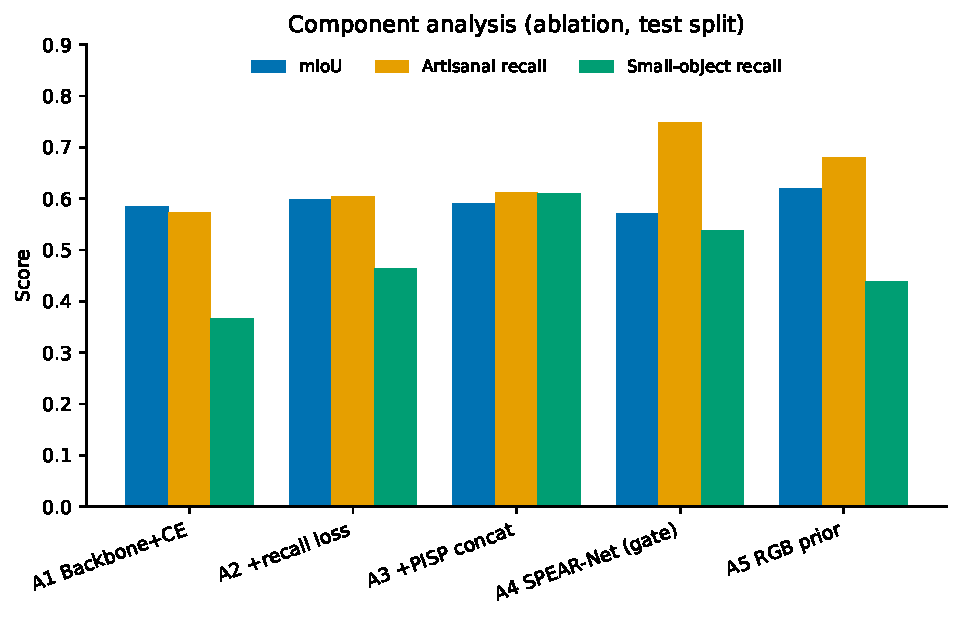
\includegraphics[width=0.78\linewidth]{fig_ablation}
\caption{Component analysis of the lightweight variants (A1--A5): mIoU and the two
mining-class IoUs. The industrial class benefits most from the recall-weighted objective
(A1$\rightarrow$A2) and the spectral prior (A2$\rightarrow$A3/A4).}
\label{fig:ablbars}
\end{figure}

\begin{table}[t]
\centering
\caption{Component analysis of SPEAR-Net (shared backbone and budget). ``Prior'' denotes
the spectral-prior integration mode; ``RGB'' uses colour indices from the visible bands
only.}
\label{tab:ablation}
\small
\setlength{\tabcolsep}{5pt}
\begin{tabular}{l l ccc cc}
\toprule
Configuration & Prior & mIoU & Recall & \multicolumn{3}{c}{Per-class IoU}\\
\cmidrule(lr){5-7}
 & & & & bg & artisanal & industrial \\
\midrule
Backbone + cross-entropy        & ---            & 0.634 & 0.714 & \best{0.910} & \best{0.533} & 0.459 \\
\;+ recall-weighted loss        & ---            & 0.640 & 0.748 & 0.907 & 0.526 & 0.487 \\
\;+ PISP (concat)               & concat, 6-band & \best{0.642} & 0.764 & 0.904 & 0.517 & 0.504 \\
\;+ PISP gate + edge (full)     & gate, 6-band   & 0.639 & \best{0.784} & 0.901 & 0.515 & 0.500 \\
\;\;\;RGB prior variant         & gate, 3-band   & 0.628 & 0.755 & 0.899 & 0.520 & 0.465 \\
\bottomrule
\end{tabular}
\end{table}

\subsection{Where errors concentrate: area-stratified recall}\label{sec:results-area}
Table~\ref{tab:area} reports SPEAR-Net's recall stratified by ground-truth object size. As
expected from the field-wide failure mode, recall rises monotonically with object size,
from \num{0.44} for small components to \num{0.92} for large ones
(Fig.~\ref{fig:areabars}). The small-object regime is therefore the dominant remaining
error source, which is consistent with the difficulty of fragmented artisanal sites and
delineates a concrete target for future work.

\begin{figure}[t]
\centering
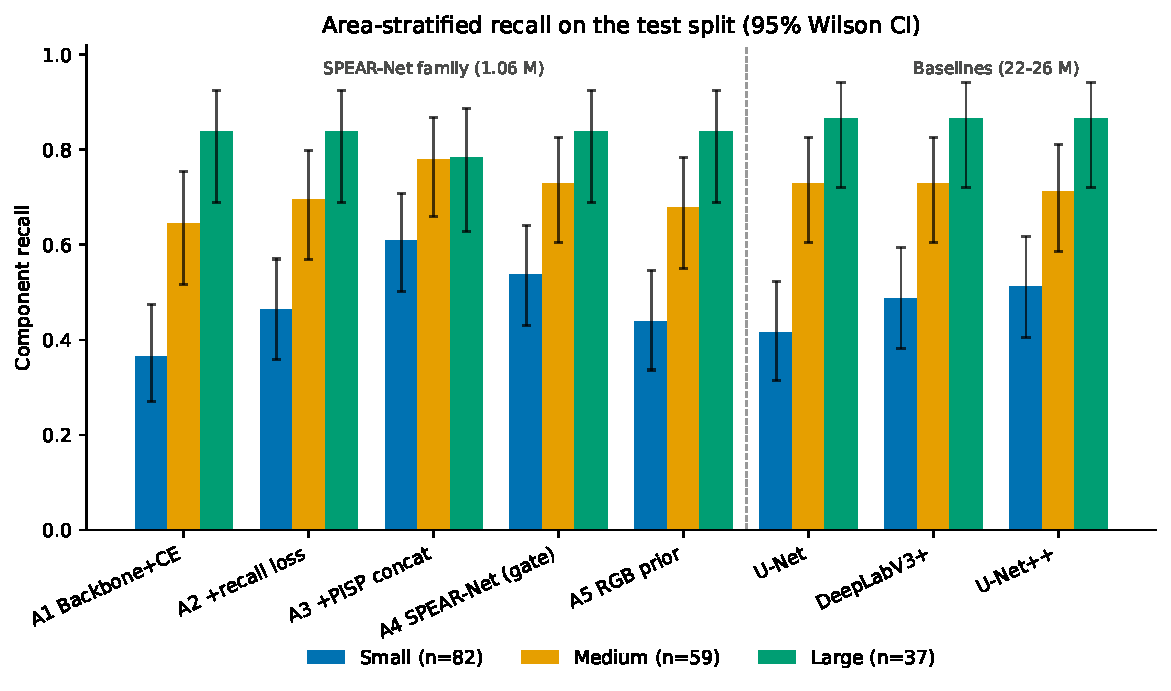
\includegraphics[width=0.5\linewidth]{fig_area_recall}
\caption{Area-stratified component recall of SPEAR-Net (Eq.~\ref{eq:areastrat}). Recall
rises monotonically with component area; small, fragmented sites remain the dominant error
mode.}
\label{fig:areabars}
\end{figure}

\begin{table}[t]
\centering
\caption{Area-stratified recall of SPEAR-Net over connected foreground components
($n$ = number of components per bin).}
\label{tab:area}
\small
\begin{tabular}{lccc}
\toprule
Object size & Small ($<32^2$) & Medium & Large ($\geq96^2$) \\
\midrule
Recall & 0.44 & 0.80 & 0.92 \\
$n$    & 68   & 49   & 51 \\
\bottomrule
\end{tabular}
\end{table}

\subsection{Geographic generalization}\label{sec:results-gen}
Table~\ref{tab:gen} reports the leave-one-region-out experiment in which Asia and Oceania
are held out of training. SPEAR-Net scores \num{0.734} mIoU on the held-out continents
versus \num{0.618} in-region, i.e.\ it does not degrade on unseen geographies in this split.
We report this as a single hold-out; a full rotation over all regions is left to future
work. The result nonetheless indicates that the learned representation is not over-fitted to
specific continents, which is important for a globally deployable monitoring tool.

\begin{table}[t]
\centering
\caption{Leave-one-region-out generalization (Asia and Oceania held out of training).}
\label{tab:gen}
\small
\begin{tabular}{lc}
\toprule
Evaluation region & mIoU \\
\midrule
In-region (training continents) & 0.618 \\
Out-of-region (held-out Asia + Oceania) & 0.734 \\
\bottomrule
\end{tabular}
\end{table}

\subsection{Qualitative results}\label{sec:results-qual}
Figure~\ref{fig:qual} shows representative predictions together with the PISP attention map.
The prior concentrates on cleared ground and pond/tailing surfaces and away from intact
vegetation, providing an interpretable rationale for each detection; Figure~\ref{fig:priors}
visualizes the four indices for a sample scene.

\begin{figure}[t]
\centering
\includegraphics[width=\linewidth]{qualitative}
\caption{Qualitative predictions and the interpretable PISP attention map on held-out
validation chips.}
\label{fig:qual}
\end{figure}

\begin{figure}[t]
\centering
\includegraphics[width=\linewidth]{priors}
\caption{The four physically-informed spectral indices computed on the fly
(Eqs.~\ref{eq:ndvi}--\ref{eq:bsi}).}
\label{fig:priors}
\end{figure}

% =====================================================================
\section{Discussion}\label{sec:discussion}

\paragraph{Interpretation.}
The central finding is an accuracy--efficiency trade-off: SPEAR-Net retains approximately
\num{98}\,\% of the best baseline's mIoU and matches its recall while being one to two orders
of magnitude cheaper in parameters and FLOPs. For continental-scale or free-tier
deployment---where inference cost, not a fraction of a mIoU point, is the binding
constraint---this trade-off is the practically relevant result. The recall-oriented
objective is effective: recall improves substantially over a plain cross-entropy backbone,
and both mining scales are recovered rather than collapsing to background, which is the
failure repeatedly reported for imbalanced mining data.

\paragraph{On the spectral prior and its integration.}
The six-band spectral prior consistently outperforms an RGB-only prior, which quantifies the
value of the NIR/SWIR bands for separating mining from spectrally similar background and
supports the physical motivation of Eqs.~\ref{eq:ndvi}--\ref{eq:bsi}. Between the two
integration modes, we do not claim that the learned gate improves accuracy over simple
concatenation: on mIoU they are statistically indistinguishable at this budget. The gate's
value is instead higher recall and interpretability---it yields a single, named-index-derived
attention map that explains each detection---so we present it as a recall-oriented and
explainable design choice, and report the concatenation variant as the marginally more
accurate, slightly cheaper alternative. We consider this candour a strength: it identifies
which mechanism does the work (the spectral bands and the recall objective) rather than
attributing gains to a component the data does not support.

\paragraph{Limitations.}
Three limitations bound our claims. First, we report single-run results; although the
efficiency gap is large and unambiguous, the sub-\num{0.01} mIoU differences among
lightweight variants should be read as comparable rather than ordered, and multi-seed
variance estimates would further strengthen the ablation. Second, SPEAR-Net does not exceed
the heavier baselines on mIoU; the contribution is parity at a fraction of the cost, not
accuracy superiority. Third, the generalization evidence is a single region hold-out; a full
leave-one-region-out rotation, and evaluation of the baselines under the same protocol,
would substantiate a stronger cross-continent claim. The dominant remaining error is on
small, fragmented objects (Table~\ref{tab:area}), which points to multi-scale or
super-resolution extensions as the most promising direction.

% =====================================================================
\section{Conclusions}\label{sec:conclusion}
We introduced SPEAR-Net, a lightweight, spectrally grounded, recall-optimized network for
segmenting artisanal and industrial mining in global Sentinel-2 imagery. Trained on a
compact, expert-verified dataset with an explicit scale label, SPEAR-Net matches strong
convolutional baselines to within about \num{1.3} mIoU points and at comparable recall while
using \num{20}--\num{25}$\times$ fewer parameters and \num{30}--\num{60}$\times$ fewer FLOPs,
recovers both mining scales without background collapse, and does not degrade on held-out
continents in a leave-one-region-out test. Its explainable spectral-prior attention makes
each detection interpretable in terms of named remote-sensing indices. Because it is small,
fast and free-tier trainable, SPEAR-Net is well suited to large-area mining surveillance;
future work will target the small-object regime, multi-seed and full region-rotation
evaluation, and transfer to auxiliary ASM domains.

% =====================================================================
\section*{Declarations}
\small
\noindent\textbf{Funding.} [To be completed.]\\
\noindent\textbf{Competing interests.} The authors declare no competing interests.\\
\noindent\textbf{Data availability.} The mining annotation dataset is publicly available
\citep{jasansky2024dataset}; Sentinel-2 imagery is openly available and was accessed via an
open cloud archive \citep{planetarycomputer}.\\
\noindent\textbf{Code availability.} Code, configurations and the data-preparation pipeline
are released at \url{https://github.com/prakhar443/illegal_mining}.\\
\noindent\textbf{Author contributions.} [To be completed.]

% =====================================================================
% For Springer submission use \bibliographystyle{spbasic} (ships with the Springer Nature
% template). plainnat is used here so the manuscript compiles standalone anywhere.
\bibliographystyle{plainnat}
\bibliography{references}

\end{document}
